




\section{Context/Problem Statement} \label{sec:context}
The present section introduces the synergy requirement that we aim to 
preserve while reasoning about performance requirements for access control policies and clarifies the motivation for the work presented in this paper.

\subsection{Synergy Requirement related to the considered Access Control Architecture}

Managing access control policies is one of the most challenging issues faced by organizations. 
Frequent changes in access control systems may be required to meet business needs. An access control system has to handle some specific 
requirements like role swapping when employees are given temporary assignments, changes in the policies and procedures, 
new assets, users and job positions in the organization.
All these facts make access control architectures very difficult to manage, and plead in favor of a simple access control architecture that can easily 
handle changes in access control systems. 

Today's access control scenarios involve an access control policy which is modeled, analyzed and implemented as a separate component 
encapsulated in a PDP. Figure \ref{pep-pdp} illustrates the interactions between the PEPs and the PDP: the PEP calls the PDP to 
retrieve an authorization decision based on the PDP encapsulated policy. This authorization decision is made through the evaluation of rules in the policy. 
Subsequently, an authorization decision (permit/deny) is returned to the PEP.
The separation between the PEP and the PDP in access control systems simplifies policy management across many heterogeneous systems and enables to avoid
 potential risks arising from incorrect policy implementation, when the policy is hardcoded inside the business logic.

\begin{figure}[!h]
\begin{center}
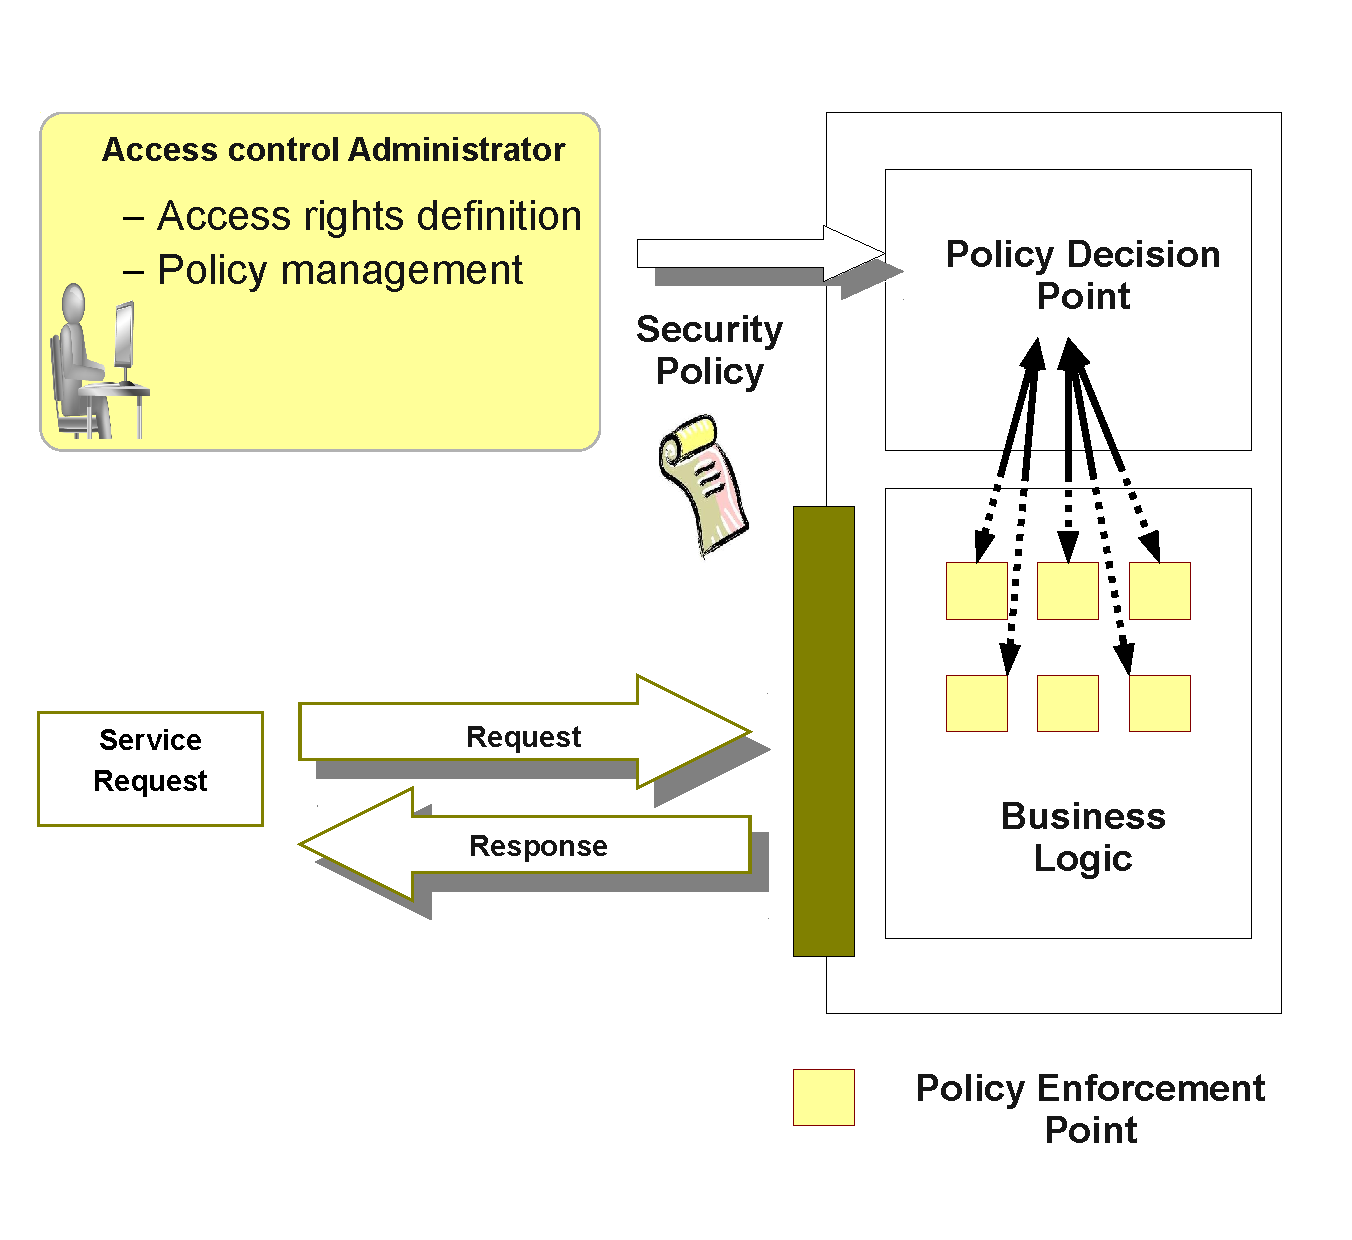
\includegraphics[width=9cm, height=8cm]{business-logic}
\caption{Access Control Request Processing}
\label{pep-pdp}
\end{center}
\end{figure}

Along with the reasoning about performance, we propose to maintain the simplicity of the access control architecture whose model 
is presented in Figure \ref{model}. In this model, a set of business processes, which comply to users' needs, are encapsulated in a given business logic 
which is enforced by multiple PEPs. Conceptually, the decision is decoupled from the enforcement and involves a decision making process in which each PEP 
interacts with one single PDP, thus a single XACML policy is evaluated to provide the suitable response for an access control request provided by a given PEP. 
\begin{figure}[!h]
\begin{center}
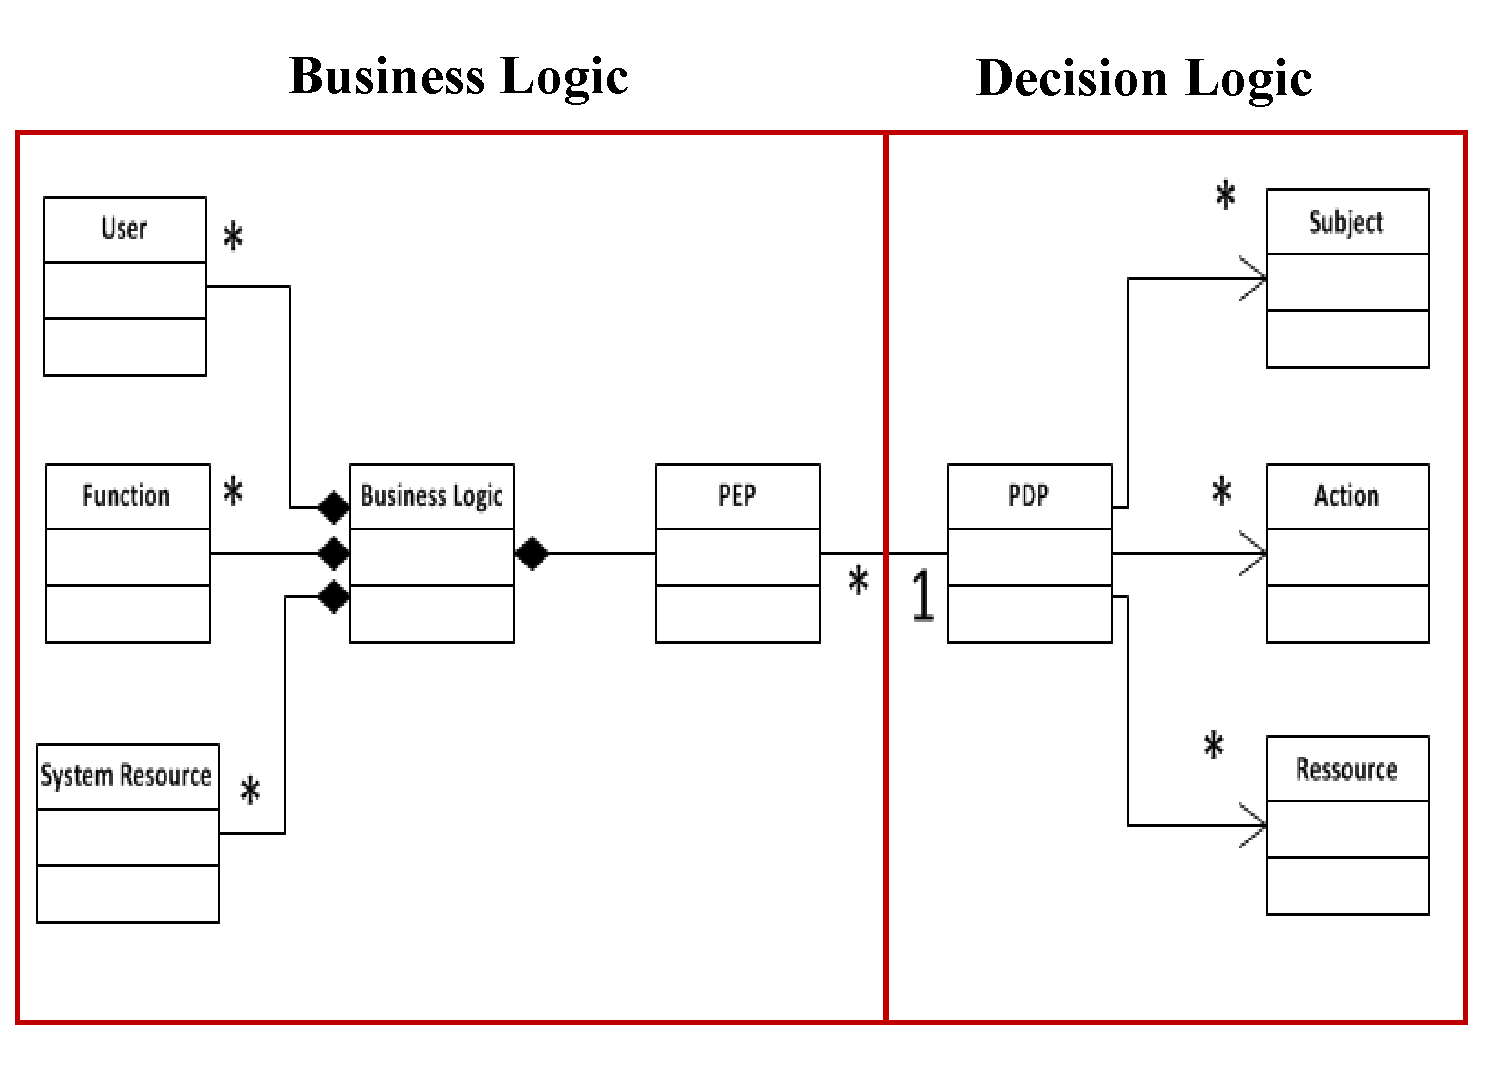
\includegraphics[height=5.5cm,width=8.5cm]{model}
\caption{The Access Control Model}
\label{model}
\end{center}
\end{figure}

Considering a single XACML policy file for each initiating PEP enables to ease policies management and to maintain a simple architecture 
in which a given PEP is mapped to a fixed PDP at each decision making process. In this work, We define the synergy requirement in the access control 
architecture by the strict mapping that exists between the enforcement of access control at the code level and the PDP. In others words, a system is synergic if 
its PEPs are predefined to be used for a particular policy in the system before deployment. 
The goal behind maintaining a single policy related to each PEP in the system is to keep a strong traceability between what has been specified by the 
policy at the decision level and the internal security mechanisms enforcing this policy at the business logic level. In such setting, 
when access control policies are updated or removed, the related PEPs can be easily located and removed and thus the application is updated synchronously 
with the policy changes. 

\subsection{XACML Access Control Policies and Performance Issues}

In this paper, we focus on access control policies specified in the eXtensible Access Control Modeling Language (XACML)~\cite{sunxacml}.
XACML is an XML-based standard policy specification language that defines a syntax of access control policies and
request/response. \\XACML enables policy authors to externalize access control policies for the sake of interoperability since access control policies can be designed 
independently from the underlying programming language or platform. Such flexibility enables to easily update access control policies to comply with new requirements.

An XACML is constructed as follows.
A \CodeIn{policy set} element consists of a sequence of \CodeIn{policy elements}, a combining algorithm, and
a \CodeIn{policy target} element. A \CodeIn{policy element} is expressed through a target, a set of \CodeIn{rules}, and a rule combining algorithm. 
A \CodeIn{target} element consists of the set of resources, subjects, and actions to which a rule is applicable. A \CodeIn{rule} consists of a 
\CodeIn{target} element, a \CodeIn{condition} element, and an \CodeIn{effect}. A \CodeIn{condition} element is a boolean expression that specifies the
environmental context (e.g., time and location restrictions) in which the rule applies.
Finally, an \CodeIn{effect} is the rule's authorization decision, which is either permit or deny.

Given a request, a PDP evaluates the request against the \CodeIn{rules} in the policy by matching resources, subjects, actions, and condition in the request.
More specifically, an XACML request encapsulates attributes, which define which subject requests to take action on which resource in which
condition (e.g., subject Bob requests to borrow a book).
%This can be under/not a condition.
Given a request, that satisfies \CodeIn{target} and \CodeIn{condition} elements in a rule, the rule's effect
is taken as the decision.
If the request does not satisfy \CodeIn{target} and \CodeIn{condition} elements in any rule, its response yields the ``NotApplicable'' decision.

When more than one rule is applicable to a request, the combining algorithm helps determine which rule's effect can be finally given as the decision for the request.
For example, given two rules, that are applicable to the same request and provide different decisions,
the permit-overrides algorithm prioritizes a permit decision over the other decisions.
More precisely, when using the permit-overrides algorithm, the policy evaluation produces one of the following three decisions: 

\begin{itemize}
\item Permit if at least one permit rule is applicable for a request.
\item Deny if no permit rule is applicable and at least one deny rule is applicable for a request.
\item NotApplicable if no rule is applicable for a request.
\end{itemize}

Figure \ref{figur1} shows a simplified XACML policy that denies subject Bob to borrow a book.

%\fontsize{5}{5}
\begin{figure}[!h]
\begin{center}
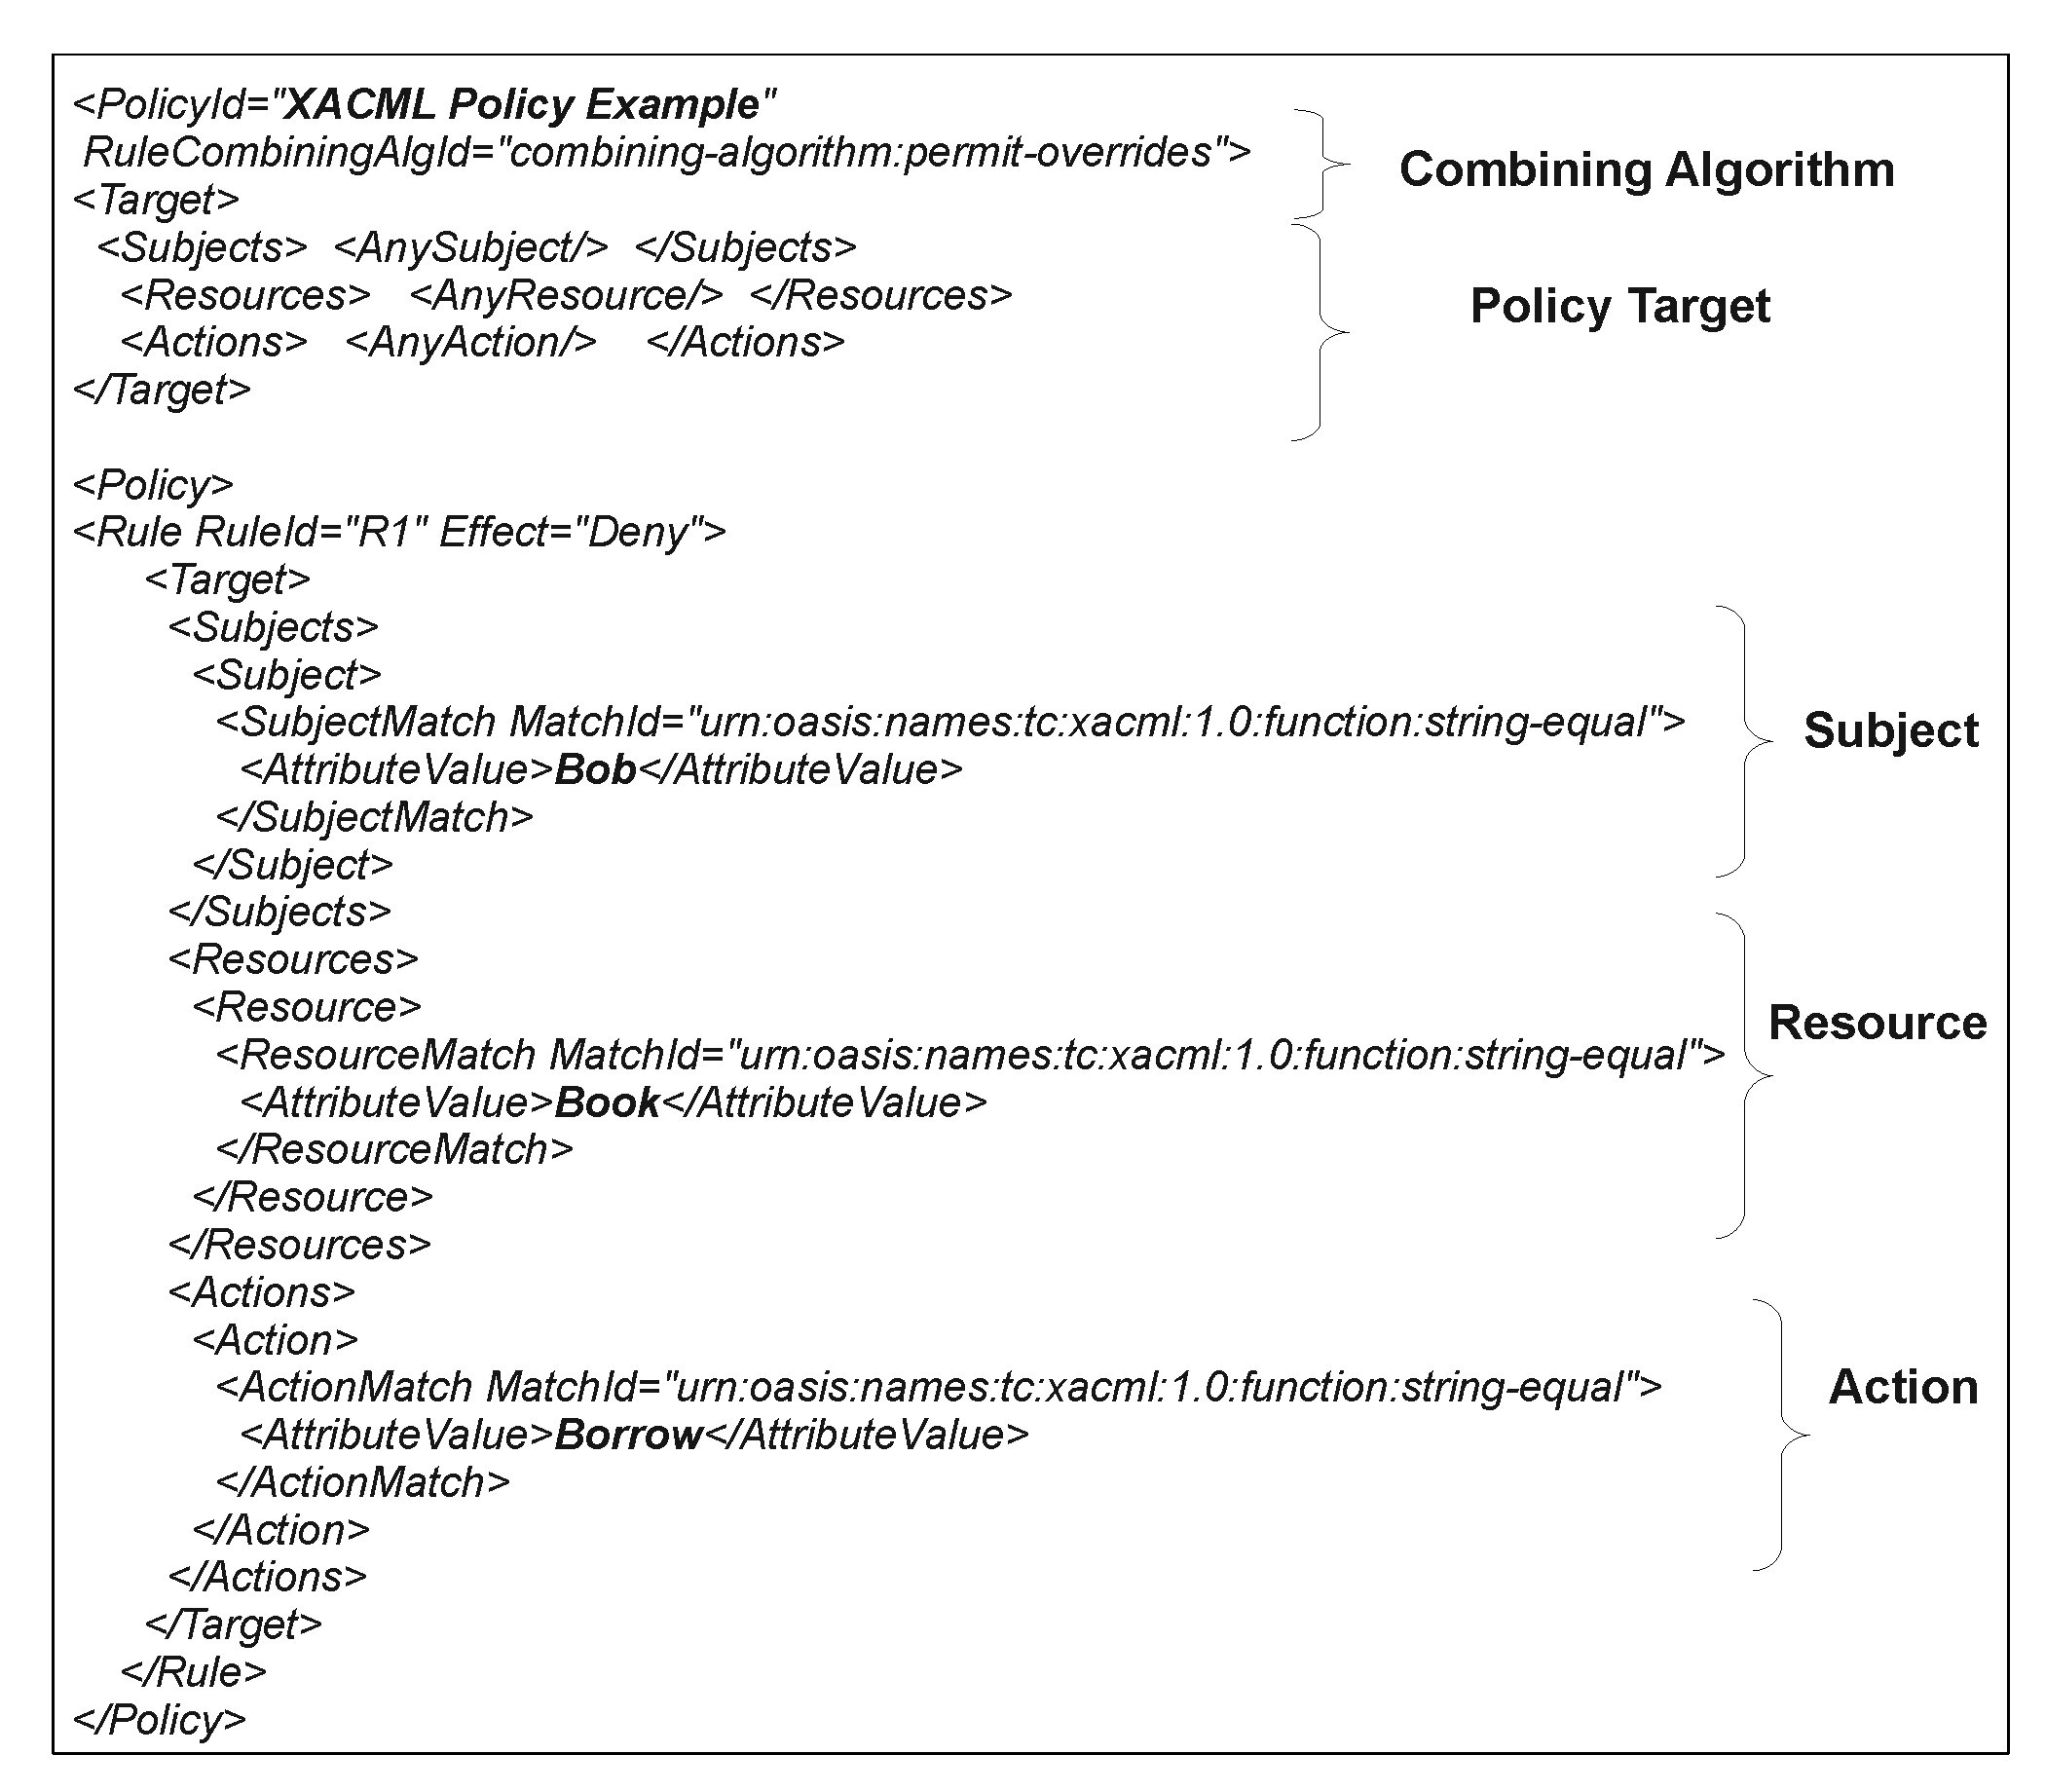
\includegraphics[width=8.6cm]{xacml}
\caption{XACML Policy Example}
\label{figur1}
\end{center}
\end{figure}

 
\Comment{ 
\begin{figure}[!h]%{t}
%\begin{figure}[firstnumber=100]
\begin{CodeOut}
\begin{alltt}
\small
 1 <PolicySet PolicyId="\textbf{An Example Policy Set}" PolicyCombAlgId="\textbf{Permit-overrides}">
 2 <Target/> 
 3  <Policy PolicyId="\textbf{An Example Policy}" RuleCombAlgId="\textbf{Permit-overrides}">
 4   <Target/>
 5    <Rule RuleId="\textbf{1}" Effect="\textbf{Deny}">
 6      <Target>
 7        <Subjects><Subject> \textbf{Bob} </Subject></Subjects>
 8        <Resources><Resource> \textbf{BOOK} </Resource></Resources>
 9        <Actions><Action> \textbf{BORROW} </Action></Actions>
10      </Target>
11	    <Condition>
12        <AttributeValue> \textbf{DEFAULT} </AttributeValue>
13      </Condition>
14    </Rule>
15      <!-- A final, "fall-through" rule that always Denies -->
16    <Rule RuleId="\textbf{FinalRule}" Effect="\textbf{Deny}"/>
17  </policy>
18 </policySet>
\end{alltt}
\end{CodeOut}
\vspace*{-3.0ex} \caption{An XACML Policy Example}
 \label{figur1}
\end{figure}
}
 

%\centering
%\figure[DREF metamodel\label{fig:drefMM}]
%        {\includegraphics[width=0.5\textwidth]{figure/drefMM}}
%\figure[SETER Process: Security Testing for Resilient Systems 
%\label{fig:seter}] {\includegraphics[width=0.49\textwidth]{figure/seter}}
%\caption{DREF and SETER: Conceptual and Operational Frameworks for evaluating resilient systems}
%\end{figure*}


Recently, an XACML policy becomes more complex to handle increasing complexity of organizations in terms of structure, relationships, activities, and access control requirements. In such a situation, the policy often consists of a large number of rules to specify policy behaviors for various resources, users and actions in the organizations.
In policy-based systems, policy authors manage centralized a single PDP loaded with a single policy to govern all of system resources. 
However, due to a large number of rules for evaluation, this centralization raises performance concerns related to request evaluation time for XACML access control policies and may 
degrade the system efficiency and slow down the overall business processes. 

We present following three main factors, that may cause to degrade XACML request evaluation performance: 

\begin{itemize}
\item An XACML policy may contain various attribute elements including \CodeIn{target} elements. Retrieval of
attribute values in the \CodeIn{target} elements for request evaluation may increase the evaluation time.
\item A \CodeIn{policy set} consists of a set of policies. Given a request, a PDP determines the final authorization decision (i.e., effect) of the whole \CodeIn{policy set} after combining all the applicable rules' decisions according to the request.
Computing and combining applicable rules' decisions contributes to increase the evaluation time.
\item \CodeIn{Condition} elements in rules can be complex because these elements are built from an arbitrary nesting of non-boolean functions and attributes. In such a situation, evaluating \CodeIn{condition} elements may slow down request evaluation time.
\end{itemize}

